\documentclass[a4paper,10pt]{article}
\usepackage{polski}
\usepackage[utf8]{inputenc}
\usepackage{array,floatflt,textcomp,graphicx,longtable}
%custom margins
\usepackage[left=2.5cm, top=2.5cm, bottom=3cm, right=2cm, foot=2cm, head=0.5cm]{geometry}
\usepackage{fancyhdr}
\usepackage[bookmarks=true, pdftex]{hyperref}

%styl nagłowków
\pagestyle{fancy} 
\parindent 2cm 

%opening
\title{Specyfikacja wymagań systemowych}
\author{3@KASK}

\begin{document}
\bibliographystyle{plain}


\maketitle


\begin{center}
%budowanie tabeli
\begin{tabular}{|p{7cm}|p{7cm}|}
\hline
Symbol projektu: & Opiekun projektu:   \tabularnewline 
3@KASK & Tomasz Boiński    \tabularnewline \hline
\multicolumn{2}{|l|}{Nazwa Projektu: } \tabularnewline
\multicolumn{2}{|l|}{Wizualizacja grafów za pomocą biblioteki Prefuse } \tabularnewline 
\hline
\multicolumn{2}{l}{ } \tabularnewline %pusta linijka
\hline 
Nazwa Dokumentu: & Nr wersji:   \tabularnewline 
Specyfikacja wymagań systemowych & 0.4 \tabularnewline \hline
Odpowiedzialny za dokument: & Data pierwszego sporządzenia:   \tabularnewline 
Piotr Orłowski & 15 kwietnia 2009 \tabularnewline \hline
Przeznaczenie: & Data ostatniej aktualizacji:   \tabularnewline 
DLA KLIENTA & \today \tabularnewline \hline
\end{tabular}
\end{center}


\begin{center}
\begin{tabular}{|c|p{4cm}|c|c|c|}
\multicolumn{5}{c}{\textbf{Historia dokumentu}} \tabularnewline \hline
\textbf{Wersja} & \textbf{Opis modyfikacji} & \textbf{Rozdział/strona} & \textbf{Autor modyfikacji} & \textbf{Data} \tabularnewline \hline 
1 & Stworzenie & wszystkie & Grupa projektowa & 15.04.09 \tabularnewline \hline
2 & Wpisanie celów i wymogów ogólnych  & cele & Grupa projektowa & 16.04.09\tabularnewline \hline
3 & Wpisanie funkcjonalnosci wizualizacyjnych & & Grupa projektowa & 28.04.09\tabularnewline \hline
4 & Opis wymagań & & Grupa projektowa & 05.05.09\tabularnewline \hline
\end{tabular}
\end{center}


\newpage
\tableofcontents
\newpage

\section{Cele systemu}

%Chociaż cele projektu zostały sformułowane w zleceniu projektowym, to w tym miejscu precyzuje się je z podziałem na cele biznesowe i cele funkcjonalne. Zdarza się tak, że zleceniodawca początkowo wymienia tylko cele funkcjonalne zachowując do swojej wiadomości cele biznesowe. Aby jednak właściwie rozumieć te funkcje w odpowiednim kontekście, zespół projektowy musi poznać motywacje biznesowe klienta.

\subsection{Cele biznesowe}




\begin{center}
\begin{tabular}{|m{3cm}|m{9cm}|} \hline

CB001 & Ułatwienie pracy programistom tworzącym aplikacje wizualizujące ontologie  \\ \hline
Opis: & Istnieje zapotrzebowanie na bibliotekę tłumaczącą OWL bezpośrednio na elementy graficzne.  \\ \hline
Źródło: & Wstępna specyfikacja projektu \\ \hline
Priorytet: & bardzo ważne \\ \hline
\multicolumn{2}{c}{} \\

%priorytety  00 01 10 11
%priorytety bardzo wazne, wazne, średnio ważne, mało wazne

 \hline
CB002 & Ułatwienie zakończenia projektu OCS   \\ \hline
Opis: & Moduł wizualizujący ontolgie w OCS wymaga modernizacji i rozbudowy funkcjonalności. Zapewnienie biblioteki wizualizującej ontologie ułatwi i przyspieszy ten proces.  \\ \hline
Źródło:& Klient - mgr inż. Tomasz Boiński   \\ \hline
Priorytet: & bardzo ważne \\ \hline
\multicolumn{2}{c}{} \\
 \hline
CB003 & Zwiększenie aktrakcyjności portalu OCS   \\ \hline
Opis: & Poprawa estetyki modułu wizualizującego ontologię moze przyczynic się do sukcesu portalu po jego wdrożeniu.  \\ \hline
Źródło: & Klient - mgr inż. Tomasz Boiński \\ \hline
Priorytet: & mało ważne \\ \hline
\multicolumn{2}{c}{} \\
\end{tabular}

%\begin{tabular}{|m{3cm}|m{9cm}|} \hline
%CB004 &    \\ \hline
%Opis: &   \\ \hline
%Źródło: &  \\ \hline
%Priorytet: & \\ \hline
%\end{tabular}

\end{center}

\subsection{Cele funkcjonalne}

%Cele funkcjonalne wymieniają główne funkcje, które ma spełniać system.

\begin{center}

\begin{tabular}{|m{3cm}|m{9cm}|} \hline

CF001 & Intuicyjne API \\ \hline
Opis: & Na podstawie subiektywnej opinii kilku zewnętrznych osób nie należących do zespołu projektowego oraz oceny opiekuna projektu API powinno zostać uznane za nadające się do użytku. \\ \hline
Źródło: & Klient - mgr inż. Tomasz Boiński \\ \hline
Priorytet: & średnio ważne  \\ \hline
\multicolumn{2}{c}{} \\

 \hline
CF002 & Dobra dokumentacja \\ \hline
Opis: & Przygotowanie dokumentacji w Javadoc ułatwi pracę użytkownikom biblioteki. \\ \hline
Źródło: & Klient - mgr inż. Tomasz Boiński  \\ \hline
Priorytet: & bardzo ważne \\ \hline

\multicolumn{2}{c}{} \\
 \hline
CF003 & Wizualizacja ontologii \\ \hline
Opis: & Stworzenie biblioteki, która pozwoli na wizualizacje obiektów OWL API przy użyciu odpowiedniej biblioteki graficznej. \\ \hline
Źródło:  & Specyfikacja projektu  \\ \hline
Priorytet: & bardzo ważne \\ \hline

\multicolumn{2}{c}{} \\
 \hline
CF004 & Umożliwienie graficznej edycji i dodawania obiektów OWL API \\ \hline
Opis: &  Dostarczenie tej funkcjonalności ułatwi tworzenie programów z interfejsem pozwalającym na edycję ontologii zapisanych w OWL API. \\ \hline
Źródło: & Klient - mgr inż. Tomasz Boiński \\ \hline
Priorytet: & średnio ważne \\ \hline
\multicolumn{2}{c}{} \\


 \hline

CF005 & Udostępnienie informacji do debuggowania  \\ \hline
Opis: &  Biblioteka powinna wysyłać komunikaty informacyjne, ostrzegawcze oraz informujace o błędach na strumień udostępniony użytkownikowi.  \\ \hline
Źródło: & Standard tworzenia biblioteki \cite{artOstandardach} \\ \hline
Priorytet: & średnio ważne \\ \hline

\end{tabular}

\end{center}

\section{Otoczenie systemu}

%Zespół projektowy musi poznać otoczenie, w jakim ma pracować system. Z rozmów z klientem powinno dać się wyszczególnić użytkowników oraz systemy zewnętrzne. Jeśli się nie da, to otoczenie systemu trzeba będzie zdefiniować w trakcie analizy funkcjonalnej.

\subsection{Użytkownicy}

Specyfika projektu nie definiuje użytkowników systemu.

%\begin{tabular}{|m{3cm}|m{9cm}|} \hline

%Tutaj jest ID & A tutaj nazwa \\ \hline
%Opis: &  \\ \hline
%Potrzeby: &  \\ \hline
%Zadania: &  \\ \hline
%Źródło: &  \\ \hline
%Priorytet: &  \\ \hline

%\end{tabular}


\subsection{Systemy zewnętrzne}

Specyfika systemu nie wymaga definiowaia systemów zewnętrznych.

%\begin{center}
%\begin{tabular}{|m{3cm}|m{9cm}|} \hline

%Tutaj jest ID & A tutaj nazwa \\ \hline
%Opis: &  \\ \hline
%Interfejsy: &  \\ \hline
%Źródło: &  \\ \hline
%Priorytet: &  \\ \hline

%\end{tabular}
%\end{center}

\section{Przewidywane komponenty systemu}

%Wyszczególnienie komponentów systemu powinno pomóc w uzyskaniu kompletności wymagań. Trzeba wówczas sprawdzić, czy każdy komponent ma jakieś wymagania (zwłaszcza funkcjonalne). W przypadku bardziej złożonego systemu może być konieczne wyszczególnienie podsystemów.

\subsection{Podsystemy}
Specyfika projektu sprawia, że podsystemy nie będa rozpatrywane.

\subsection{Komponenty sprzętowe}
Specyfika projektu sprawia, że komponenty sprzętowe nie będa rozpatrywane. 

\subsection{Programowe}

\begin{center}
\begin{tabular}{|m{3cm}|m{9cm}|} \hline

KS001 & Prefuse \\ \hline
Opis: &  Biblioteka graficzna do wizualizacji grafów w języku Java\\ \hline
Powiązania: &  \\ \hline
Źródło: & Specyfikacja projektu \\ \hline
Priorytet: & bardzo ważne \\ \hline

\end{tabular}
\end{center}

\section{Wymagania funkcjonalne}

%Wymagania funkcjonalne stanowią mocno rozbudowaną część specyfikacji. Można je podzielić na grupy dotyczące różnych zadań, różnych użytkowników (systemów zewnętrznych) albo różnych komponentów.

\begin{center}

\begin{tabular}{|m{3cm}|m{9cm}|} \hline

WF001 & Udostępnienie kilku algorytmów wizualizacji \\ \hline
Opis: & Biblioteka powinna udostępniać kilka trybów prezentacji grafów (np. w formie drzewa, w formie gwiazdy i innych).    \\ \hline
Dotyczy: & CF003 \\ \hline
Źródło: & klient - mgr Tomasz Boiński \\ \hline
Powiązania: &WF002 \\ \hline
Priorytet: &  ważny\\ \hline

\multicolumn{2}{c}{} \\
 \hline

WF002 & Parametryzacja trybów wizualizacyjnych \\ \hline
Opis: & Domyślne parametry w trybach wizualizacji (takie jak długość krawędzi grafu, automatyczne układanie) powinny zostać dobrane w taki sposób, by obraz był przejrzysty, stabilny i czytelny.    \\ \hline
Dotyczy: & CF003 \\ \hline
Źródło: &  klient - mgr Tomasz Boiński\\ \hline
Powiązania: & WF001 \\ \hline
Priorytet: & średnio ważny \\ \hline

\multicolumn{2}{c}{} \\
 \hline

WF003 & Udostępnienie strumienia błędów \\ \hline
Opis: &   Biblioteka będzie udostępniać strumień danych, w którym znajdą się komunikaty o błędach. Strumień ten będzie mógł zostać wykorzystany przez użytkownika. \\ \hline
Dotyczy: &  CF005  \\ \hline
Źródło: & klient - mgr inż. Tomasz Boiński \\ \hline
Powiązania: & \\ \hline
Priorytet: & ważne \\ \hline

\end{tabular}

\end{center}

\subsection{Wymagania wizualizacji ontologii}

\begin{center}
\begin{tabular}{|m{3cm}|m{9cm}|} \hline

WF004 & Rozróżnialność podstawowych symboli  \\ \hline
Opis: &  Class, Individual, Property powinny mieć rozróżnialne symbole   \\ \hline
Dotyczy: &  CF003 \\ \hline
Źródło: &  klient - mgr inż. Tomasz Boiński\\ \hline
Powiązania: & \\ \hline
Priorytet: & bardzo ważne \\ \hline
%Projekt: & \includegraphics{myimage.png}

\multicolumn{2}{c}{} \\
 \hline

WF005 &   Rozróżnialność szczególnych typów Class\\ \hline
Opis: &   Klasa anonimowa, datatype, Thing i Nothing powinny być łatwo rozpoznawalne.  \\ \hline
Dotyczy: &  CF003 \\ \hline
Źródło: &  klient - mgr inż. Tomasz Boiński\\ \hline
Powiązania: & WF004 \\ \hline
Priorytet: &  ważne \\ \hline

\multicolumn{2}{c}{} \\
 \hline

WF006 &  Rozróżnialność związków między klasami (Class), instancjami (Individual) oraz predykatami (Property)\\ \hline
Opis: & Rózne symobole dla equivalentClass, disjointWith, subClassOf, sameAs, differentFrom, allDifferent, oneOf, unionOf, intersectionOf, complementOf, subProperty, equivalentProperty, hasProperty.   \\ \hline
Dotyczy: &  CF003\\ \hline
Źródło: &  klient - mgr inż. Tomasz Boiński \\ \hline
Powiązania: & WF005, WF004 \\ \hline
Priorytet: & ważne \\ \hline

\multicolumn{2}{c}{} \\
 \hline

WF007 & Rozróżnialność ograniczeń predykatów (Restrictions) \\ \hline
Opis: & Wyróżnić kardynalność (cardinality), domeny (domains) predykatów, inverseOf, właściwości predykatów (transitive, symmetric, functional, inverseFunctional). \\ \hline
Dotyczy: &  CF003\\ \hline
Źródło: &  klient - mgr inż. Tomasz Boiński \\ \hline
Powiązania: & WF004\\ \hline
Priorytet: & ważne \\ \hline

\multicolumn{2}{c}{} \\
 \hline

WF008 &  Podświetlanie wybranych związków i powiazań.\\ \hline
Opis: &   Podświetlać subklasy danej klasy po ich wybraniu myszką po zdefiniowanym zdarzeniu; podobnie subproperty i complex class. \\ \hline
Dotyczy: &  CF003\\ \hline
Źródło: &  klient - mgr inż. Tomasz Boiński \\ \hline
Powiązania: & WF006\\ \hline
Priorytet: & mało ważne \\ \hline

\multicolumn{2}{c}{} \\
 \hline

WF009 & Możliwość definiowania zdarzeń. \\ \hline
Opis: &   Użytkownik będzie mógł pod uchwyty zdarzeń podpinać własne funkcje obsługi. \\ \hline
Dotyczy: & CF003, CF004  \\ \hline
Źródło: & klient - mgr inż. Tomasz Boiński \\ \hline
Powiązania: & \\ \hline
Priorytet: & mało ważne \\ \hline

\end{tabular}

\end{center}

\subsection{Projekt wizualizacji}
 
\begin{longtable}{|c|c|p{7cm}|} \hline
Identyfikator: & Nazwa & Wizualizacja \\ \hline

PW001: & Thing &  
 \scalebox{0.30}{
\includegraphics{elementyGraficzne/drobne/thing.png}}
 % class.png: 194x86 pixel, 90dpi, 5.48x2.43 cm, bb=0 0 155 69
 \\ \hline

PW002: & Nothing &  
 \scalebox{0.30}{
\includegraphics{elementyGraficzne/drobne/nothing.png}}
 % class.png: 194x86 pixel, 90dpi, 5.48x2.43 cm, bb=0 0 155 69
 \\ \hline

PW003: & Class &  
 \scalebox{0.30}{
\includegraphics{elementyGraficzne/drobne/class.png}}
 % class.png: 194x86 pixel, 90dpi, 5.48x2.43 cm, bb=0 0 155 69
 \\ \hline

PW004: & Individual &  
 \scalebox{0.30}{
\includegraphics{elementyGraficzne/drobne/individual.png}}
 % class.png: 194x86 pixel, 90dpi, 5.48x2.43 cm, bb=0 0 155 69
 \\ \hline

PW005: & Property &  
 \scalebox{0.30}{
\includegraphics{elementyGraficzne/drobne/property.png}}
 % class.png: 194x86 pixel, 90dpi, 5.48x2.43 cm, bb=0 0 155 69
 \\ \hline

PW006: & Datatype &  
 \scalebox{0.30}{
\includegraphics{elementyGraficzne/drobne/datatype.png}}
 % class.png: 194x86 pixel, 90dpi, 5.48x2.43 cm, bb=0 0 155 69
 \\ \hline

PW007: & Anonymous Class &  
 \scalebox{0.30}{
\includegraphics{elementyGraficzne/drobne/anonymousClass.png}}
 % class.png: 194x86 pixel, 90dpi, 5.48x2.43 cm, bb=0 0 155 69
 \\ \hline

PW008: & Subclass &  
 \scalebox{0.30}{
\includegraphics{elementyGraficzne/drobne/subclass.png}}
 % class.png: 194x86 pixel, 90dpi, 5.48x2.43 cm, bb=0 0 155 69
 \\ \hline

PW009: & instanceOf &  
 \scalebox{0.30}{
\includegraphics{elementyGraficzne/drobne/instanceOf.png}} \newline
 \scalebox{0.30}{
\includegraphics{elementyGraficzne/drobne/instanceOfDatatype.png}}
 % class.png: 194x86 pixel, 90dpi, 5.48x2.43 cm, bb=0 0 155 69
 \\ \hline

PW010: & equivalentClass &  
 \scalebox{0.30}{
\includegraphics{elementyGraficzne/drobne/equivalentClass.png}}
 % class.png: 194x86 pixel, 90dpi, 5.48x2.43 cm, bb=0 0 155 69
 \\ \hline

PW011: & disjointWith &  
 \scalebox{0.30}{
\includegraphics{elementyGraficzne/drobne/disjointWith.png}}
 % class.png: 194x86 pixel, 90dpi, 5.48x2.43 cm, bb=0 0 155 69
 \\ \hline

PW012: & differentFrom / allDifferent &  
 \scalebox{0.30}{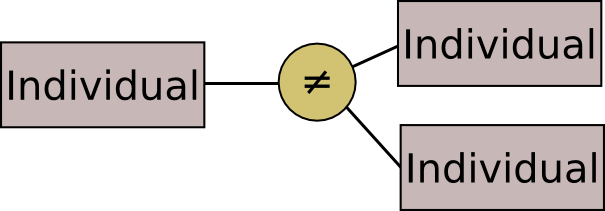
\includegraphics{elementyGraficzne/drobne/allDifferent.png}}
 % class.png: 194x86 pixel, 90dpi, 5.48x2.43 cm, bb=0 0 155 69
 \\ \hline

PW013: & sameAs &  
 \scalebox{0.30}{
\includegraphics{elementyGraficzne/drobne/sameAs.png}}
 % class.png: 194x86 pixel, 90dpi, 5.48x2.43 cm, bb=0 0 155 69
 \\ \hline

PW014: & oneOf &  
 \scalebox{0.30}{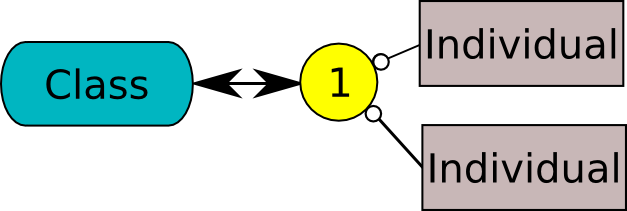
\includegraphics{elementyGraficzne/drobne/oneOf.png}}
 % class.png: 194x86 pixel, 90dpi, 5.48x2.43 cm, bb=0 0 155 69
 \\ \hline

PW015: & unionOf &  
 \scalebox{0.30}{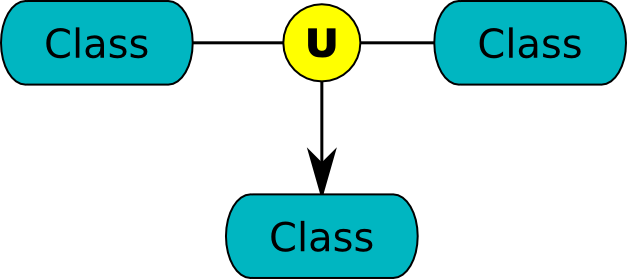
\includegraphics{elementyGraficzne/drobne/unionOf.png}}
 % class.png: 194x86 pixel, 90dpi, 5.48x2.43 cm, bb=0 0 155 69
 \\ \hline

PW016: & intersectionOf &  
 \scalebox{0.30}{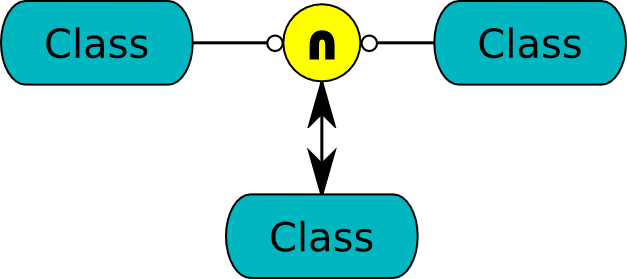
\includegraphics{elementyGraficzne/drobne/intersectionOf.png}}
 % class.png: 194x86 pixel, 90dpi, 5.48x2.43 cm, bb=0 0 155 69
 \\ \hline

PW017: & complementOf &  
 \scalebox{0.30}{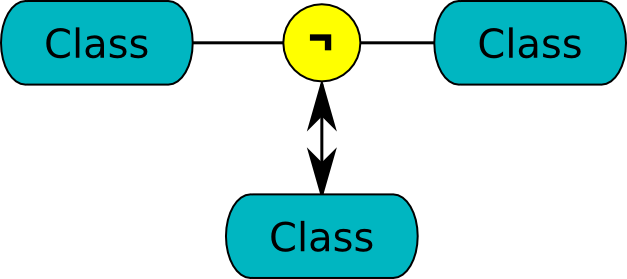
\includegraphics{elementyGraficzne/drobne/complementOf.png}}
 % class.png: 194x86 pixel, 90dpi, 5.48x2.43 cm, bb=0 0 155 69
 \\ \hline

PW018: & subProperty &  
 \scalebox{0.30}{
\includegraphics{elementyGraficzne/drobne/subProperty.png}}
 % class.png: 194x86 pixel, 90dpi, 5.48x2.43 cm, bb=0 0 155 69
 \\ \hline

PW019: & inverseOf (property) &  
 \scalebox{0.30}{
\includegraphics{elementyGraficzne/drobne/inverseOfProperty.png}}
 % class.png: 194x86 pixel, 90dpi, 5.48x2.43 cm, bb=0 0 155 69
 \\ \hline

PW020: & equivalentProperty &  
 \scalebox{0.30}{
\includegraphics{elementyGraficzne/drobne/equivalentProperty.png}}
 % class.png: 194x86 pixel, 90dpi, 5.48x2.43 cm, bb=0 0 155 69
 \\ \hline

PW021: & functionalProperty &  
 \scalebox{0.30}{
\includegraphics{elementyGraficzne/drobne/functionalProperty.png}}
 % class.png: 194x86 pixel, 90dpi, 5.48x2.43 cm, bb=0 0 155 69
 \\ \hline

PW022: & inverseFunctionalProperty &  
 \scalebox{0.30}{
\includegraphics{elementyGraficzne/drobne/inverseFunctionalProperty.png}}
 % class.png: 194x86 pixel, 90dpi, 5.48x2.43 cm, bb=0 0 155 69
 \\ \hline

PW023: & symmetricProperty &  
 \scalebox{0.30}{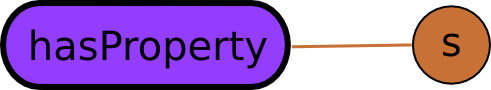
\includegraphics{elementyGraficzne/drobne/symmetricProperty.png}}
 % class.png: 194x86 pixel, 90dpi, 5.48x2.43 cm, bb=0 0 155 69
 \\ \hline

PW024: & transitiveProperty &  
 \scalebox{0.30}{
\includegraphics{elementyGraficzne/drobne/transitiveProperty.png}}
 % class.png: 194x86 pixel, 90dpi, 5.48x2.43 cm, bb=0 0 155 69
 \\ \hline

PW025: & hasProperty / domain &  
 \scalebox{0.25}{
\includegraphics{elementyGraficzne/drobne/domain.png}}
 % class.png: 194x86 pixel, 90dpi, 5.48x2.43 cm, bb=0 0 155 69
 \\ \hline

PW026: & minCardinality / maxCardinality &  
 \scalebox{0.30}{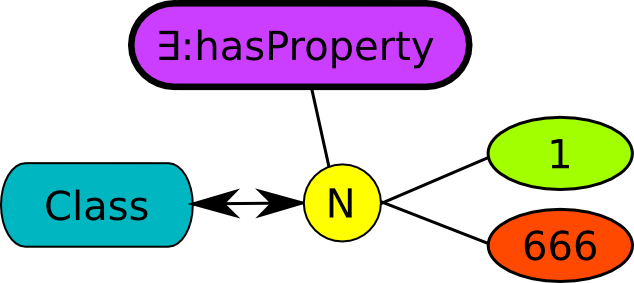
\includegraphics{elementyGraficzne/drobne/cardinalityminmax.png}}
 % class.png: 194x86 pixel, 90dpi, 5.48x2.43 cm, bb=0 0 155 69
 \\ \hline

PW027: & cardinality &  
 \scalebox{0.30}{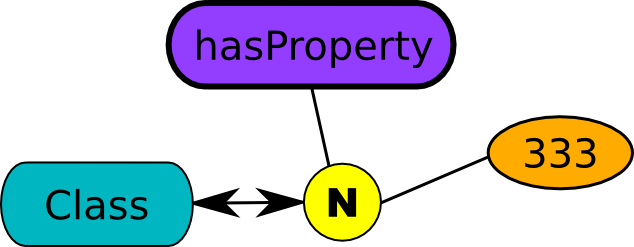
\includegraphics{elementyGraficzne/drobne/cardinality.png}}
 % class.png: 194x86 pixel, 90dpi, 5.48x2.43 cm, bb=0 0 155 69
 \\ \hline


\end{longtable}
%\scalebox{0.16}{
\includegraphics{elementyGraficzne/drobne/individual.jpg}} \\ \hline
%Projekt: & \includegraphics{myimage.png}




\section{Wymagania na dane}

%Wymagania na dane pomagają w określeniu, jakie dane będą przetwarzane w systemie. Nie trzeba precyzować wszystkich danych. Szczegóły znajdą się w projekcie bazy danych.

\begin{center}
 
\begin{tabular}{|m{3cm}|m{9cm}|} \hline

WD001 & Obsługa obiektów OWL API \\ \hline
Opis: & Biblioteka będzie przystosowana do pobierania, obróbki i zwracania obiektów OWL API. \\ \hline
Powiązania: &  \\ \hline
Źródło: & Klient - mgr inż. Tomasz Boiński  \\ \hline
Priorytet: &  bardzo ważne \\ \hline

\end{tabular}

\end{center}

\section{Wymagania jakościowe}

%Określenie wymagań jakościowych ułatwia późniejsze uzyskanie wysokiej jakości systemu. Podział wymagań jakościowych na kategorie jest związany z drzewem jakości (dotyczy wszystkich gałęzi drzewa za wyjątkiem funkcjonalności).

\subsection{Wymagania w zakresie wiarygodności}

Wymagania w zakresie wiarygodności będą rozszerzały wymagania funkcjonalne. 


\begin{center}

\begin{tabular}{|m{3cm}|m{9cm}|} \hline

WJ001 & Poprawność wizualizacji \\ \hline
Opis: & Wszystkie wizualizowane elementy powinny pochodzić z ontologii otrzymanej na wejściu programu. Program nie powinien dodawać własnych elementów (np. wywnioskowanych). \\ \hline
Powiązania: & WJ002 \\ \hline
Źródło: &  klient - mgr inż. Tomasz Boiński \\ \hline
Priorytet: & bardzo ważne \\ \hline

\multicolumn{2}{c}{} \\
 \hline

WJ002 & Kompletność wizualizacji \\ \hline
Opis: & Jeżeli biblioteka nie wizualizuje danej funkcji OWL API informacja o tym powinna znaleźć się w strumieniu błędów. \\ \hline
Powiązania: & CF005, WJ001, WD001 \\ \hline
Źródło: & klient - mgr inż. Tomasz Boiński \\ \hline
Priorytet: & ważne \\ \hline

\end{tabular}

\end{center}

\subsection{Wymagania w zakresie wydajności}

%Wymagania w zakresie wydajności będą miały zastosowanie w czasie projektowania architektury systemu.

Brak wymogów wydajnościowych ze względu na specyfikę projektu.

%\begin{tabular}{|m{3cm}|m{9cm}|} \hline

%Tutaj jest ID & A tutaj nazwa \\ \hline
%Opis: &  \\ \hline
%Powiązania: &  \\ \hline
%Źródło: klient - mgr inż. Tomasz Boiński &  \\ \hline
%Priorytet: &  \\ \hline

%\end{tabular}


\subsection{Wymagania w zakresie elastyczności}

%Wymagania w zakresie elastyczności będą miały zastosowanie w czasie wyboru koncepcji systemu.

\begin{center}

\begin{tabular}{|m{3cm}|m{9cm}|} \hline

WJ003 & Obsługiwane wersje Javy \\ \hline
Opis: & Biblioteka powinna wspierać wersje Javy 1.5 i nowsze.\\ \hline
Powiązania: &  \\ \hline
Źródło: & klient - mgr inż. Tomasz Boiński \\ \hline
Priorytet: & bardzo ważne \\ \hline

\multicolumn{2}{c}{} \\
 \hline

WJ004 & Obsługiwane wersje OWL API \\ \hline
Opis: & Powinna istnieć możliwość podpięcia zewnętrznego OWL API (wybranego przez użytkownika/programistę).\\ \hline
Powiązania: &  \\ \hline
Źródło: & klient - mgr inż. Tomasz Boiński \\ \hline
Priorytet: & bardzo ważne \\ \hline

\end{tabular}
 
\end{center}

\subsection{Wymagania w zakresie użyteczności}

%Wymagania w zakresie użyteczności będą brane pod uwagę głównie w czasie projektowania interfejsu użytkownika.

Ze względu na przyjętą metodykę wytwarzania oprogramowania zagadnienie to zostanie rozpatrzone w przyszłości.

%\begin{tabular}{|m{3cm}|m{9cm}|} \hline

%Tutaj jest ID & A tutaj nazwa \\ \hline
%Opis: &  \\ \hline
%Powiązania: &  \\ \hline
%Źródło: &  \\ \hline
%Priorytet: &  \\ \hline

%\end{tabular}


\section{Sytuacje wyjątkowe}

%Sytuacje wyjątkowe stanowią dalsze rozszerzenie wymagań funkcjonalnych i wiarygodnościowych.

Ze względu specyfikę projektu sytuacje wyjątkowe nie będą rozpatrywane.

%\begin{tabular}{|m{3cm}|m{9cm}|} \hline

%Tutaj jest ID & A tutaj nazwa \\ \hline
%Opis: &  \\ \hline
%Powiązania: &  \\ \hline
%Źródło: &  \\ \hline
%Priorytet: &  \\ \hline

%\end{tabular}


\section{Dodatkowe wymagania}

%W tym miejscu podaje się te wymagania, które nie mieszczą się w zakresie poprzednich kategorii wymagań.

\subsection{Wymagania sprzętowe}

%Wymagania sprzętowe można by umieścić w ramach specyfikacji komponentów sprzętowych, ale jeśli jest wiele komponentów sprzętowych różnych z punktu widzenia funkcjonalnego, ale o wspólnych wymaganiach sprzętowych, to można te wymagania umieścić właśnie tutaj.

Ze względu na specyfikę projektu wymagania sprzętowe nie będą rozpatrywane.

%\begin{tabular}{|m{3cm}|m{9cm}|} \hline

%Tutaj jest ID & A tutaj nazwa \\ \hline
%Opis: &  \\ \hline
%Dotyczy: &  \\ \hline
%Źródło: &  \\ \hline
%Priorytet: &  \\ \hline

%\end{tabular}


\subsection{Wymagania programowe}

%Trzeba odróżniać rzeczywiste wymagania programowe klienta od jego sugestii (np. przez podanie opcjonalnego priorytetu).

\begin{center}

\begin{tabular}{|m{3cm}|m{9cm}|} \hline

WD003 & JVM \\ \hline
Opis: & Do skorzystania z biblioteki niezbędna jest JVM.\\ \hline
Dotyczy: & CF001, CF002 \\ \hline
Źródło: & klient - mgr inż. Tomasz Boiński \\ \hline
Priorytet: & ważne \\ \hline

\end{tabular}
 
\end{center}

\subsection{Inne wymagania}
 
\begin{center}

\begin{tabular}{|m{3cm}|m{9cm}|} \hline

WD001 & Dokumentacja w javadoc \\ \hline
Opis: & Wszystkie ważne klasy i funkcje powinny mieć odpowiednią dokumentację w formacie javadoc.\\ \hline
Dotyczy: & CF001, CF002 \\ \hline
Źródło: & klient - mgr inż. Tomasz Boiński \\ \hline
Priorytet: & ważne \\ \hline

\multicolumn{2}{c}{} \\
 \hline

WI002 & Dokumentacja w języku angielskim \\ \hline
Opis: & Dokumentacja wszystkich funkcji i klas powinna posiadać angielską wersję językową.\\ \hline
Dotyczy: & CF001, CF002 \\ \hline
Źródło: & klient - mgr inż. Tomasz Boiński \\ \hline
Priorytet: & mało ważne \\ \hline

\multicolumn{2}{c}{} \\
 \hline

WI003 & Dokumentacja w języku polskim \\ \hline
Opis: & Dokumentacja wszystkich funkcji i klas powinna posiadać polską wersję językową. \\ \hline
Dotyczy: & CF001, CF002 \\ \hline
Źródło: & klient - mgr inż. Tomasz Boiński \\ \hline
Priorytet: & ważne \\ \hline

\multicolumn{2}{c}{} \\
 \hline
WI004 & Nazwy zmiennych i funkcji w języku angielskim \\ \hline
Opis: & Nazwy zmiennych i funkcji powinny zostać dobrane w języku angielskim i zgodnie ze standardami programowania w javie[standardJava].\\ \hline
Dotyczy: & CF001, CF002 \\ \hline
Źródło: & klient - mgr inż. Tomasz Boiński \\ \hline
Priorytet: & ważne \\ \hline

\end{tabular}
 
\end{center}
 
\section{Kryteria akceptacyjne}

%Tu podać kryteria, jakim zostanie poddany gotowy system przed ostatecznym jego przyjęciem.

\begin{center}

\begin{tabular}{|m{3cm}|m{9cm}|} \hline

KA001 & Spełnione są podstawowe wymagania wymienione w dokumencie SWS \\ \hline
Opis: & Spełnione są wszystkie wymagania ważne i bardzo ważne zdefiniowane w SWS. \\ \hline
Dotyczy: & W* \\ \hline
Źródło: & klient - mgr inż. Tomasz Boiński \\ \hline
Priorytet: & ważne  \\ \hline %skonsultować z klientem

\multicolumn{2}{c}{} \\
 \hline

KA002 & Biblioteka współpracuje z OWL API dostarczonym przez KASK \\ \hline
Opis: & Biblioteka współpracuje z OWL API dostarczonym przez KASK ...\\ \hline
Dotyczy: & WJ004 \\ \hline
Źródło: & klient - mgr inż. Tomasz Boiński \\ \hline
Priorytet: & ważne  \\ \hline %skonsultować z klientem

\end{tabular}
 
\end{center}

\clearpage
\phantomsection
\addcontentsline{toc}{section}{Literatura}
\bibliography{biblio}

\end{document}
